%\documentclass[show notes]{beamer}
%\documentclass[handout]{beamer}
\documentclass[]{beamer}

\usepackage{pgfpages}
\usepackage[utf8]{inputenc}
\usepackage[T1]{fontenc}
\usepackage{mathabx}
\usepackage{mathpazo}
\usepackage{eulervm}
\usepackage{natbib}
\usepackage{adjustbox}
\usepackage{booktabs}

\usepackage{caption}
\captionsetup[figure]{labelformat=empty}% redefines the caption setup of the figures environment in the beamer class.


\usetheme{Madrid}
\definecolor{uog}{rgb}{0,.5,0}
\usecolortheme[named=uog]{structure}

\mode<handout>{
    \pgfpagesuselayout{4 on 1}[letterpaper] 
    \setbeameroption{show notes}
}


% The following code uses \AtBeginSection to place a frame with the section title (\insertsectionhead) inside a beamercolorbox.
% From https://tex.stackexchange.com/questions/178800/creating-sections-each-with-title-pages-in-beamers-slides
\AtBeginSection[]{
  \begin{frame}
  \vfill
  \centering
  \begin{beamercolorbox}[sep=8pt,center,shadow=true,rounded=true]{title}
    \usebeamerfont{title}\insertsectionhead\par%
  \end{beamercolorbox}
  \vfill
  \end{frame}
}

\title[Biological Invasion of Guam]{Biological Invasion of Guam}

\author{Aubrey Moore}

\institute[University of Guam]{Cooperative Extension Service\\College of Natural and Applied Sciences\\University of Guam}

\titlegraphic{
\includegraphics[width=2cm]{big_g2.pdf}}

\date[]{WEDA/WAAESD Joint Summer Meeting, Guam\\July 11, 2018}

\begin{document}

\maketitle

\begin{frame}{Outline}
    \tableofcontents
\end{frame}

\section{Introduction}

\begin{frame}{Welcome to Guam}
    \adjincludegraphics[height=1.05\textheight,center]{Guam.jpg}
\end{frame}

\begin{frame}{HIPPO Threatens Guam's Biodiversity!}
    \adjincludegraphics[height=\textheight,center]{hippo.jpg}
\end{frame}
 
\begin{frame}{HIPPO Threatens Guam's Biodiversity!}
    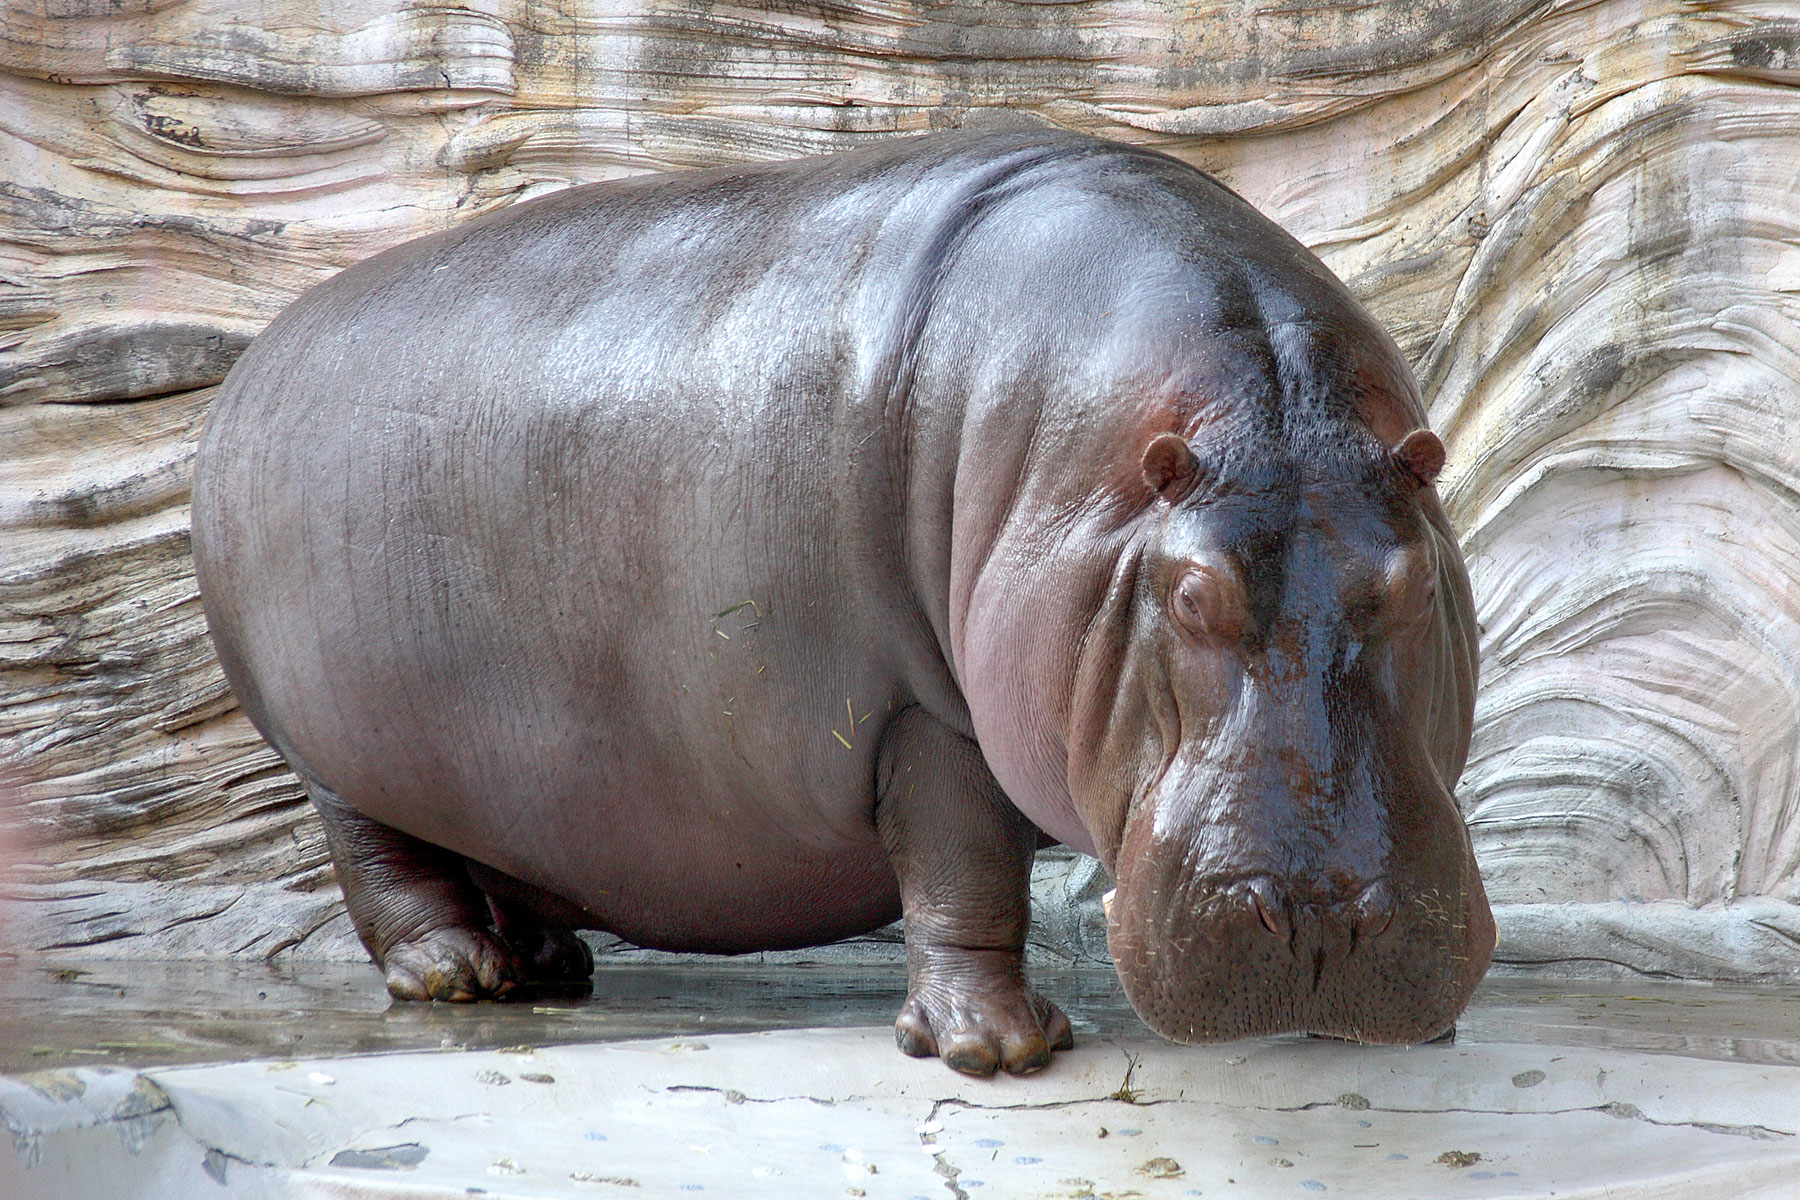
\includegraphics[height=0.5\textheight]{hippo.jpg}
    \begin{description}
        \item [\texttt{H}] Habitat loss
        \item [\texttt{I}] Invasive Species
        \item [\texttt{P}] Pollution 
        \item [\texttt{P}] Human Population
        \item [\texttt{O}] Overharvesting
    \end{description}
\end{frame}

\begin{frame}{Definition of 'Invasive Species'}
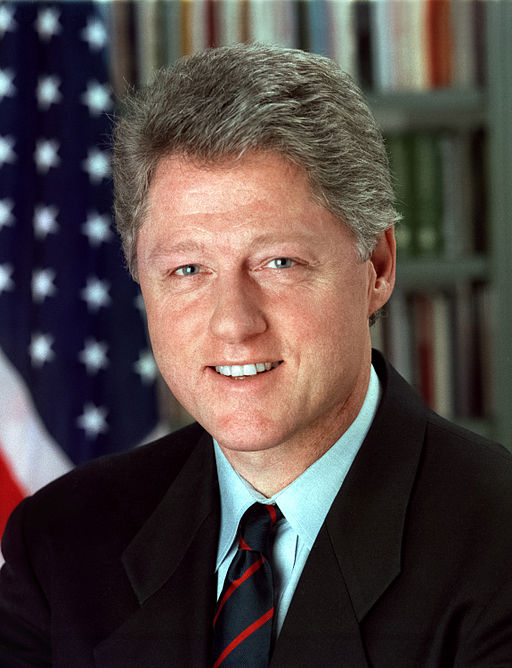
\includegraphics[height=0.4\textheight]{Bill_Clinton.jpg} \\

\textbf{Invasive species} means an \textbf{alien}
species whose introduction does or is
likely to cause economic or
environmental \textbf{harm} or harm to
human health.

\vspace{10px}
Executive Order 13112

President William Clinton

February 3, 1999

\vspace{10px}
\textbf{invasive species} were previously referred to as \textbf{exotic pests}
\end{frame}

\begin{frame}{Small tropical islands are susceptable to damage by invasive species}
\adjincludegraphics[height=0.6\textheight, center]{desert_island.jpg}
\begin{itemize}
\item no winter
\item no predators, parasites, or diseases: 'escape from natural enemies'
\end{itemize}
\end{frame}

\begin{frame}{Invasive Species Arrival Rate}
	\begin{figure}
		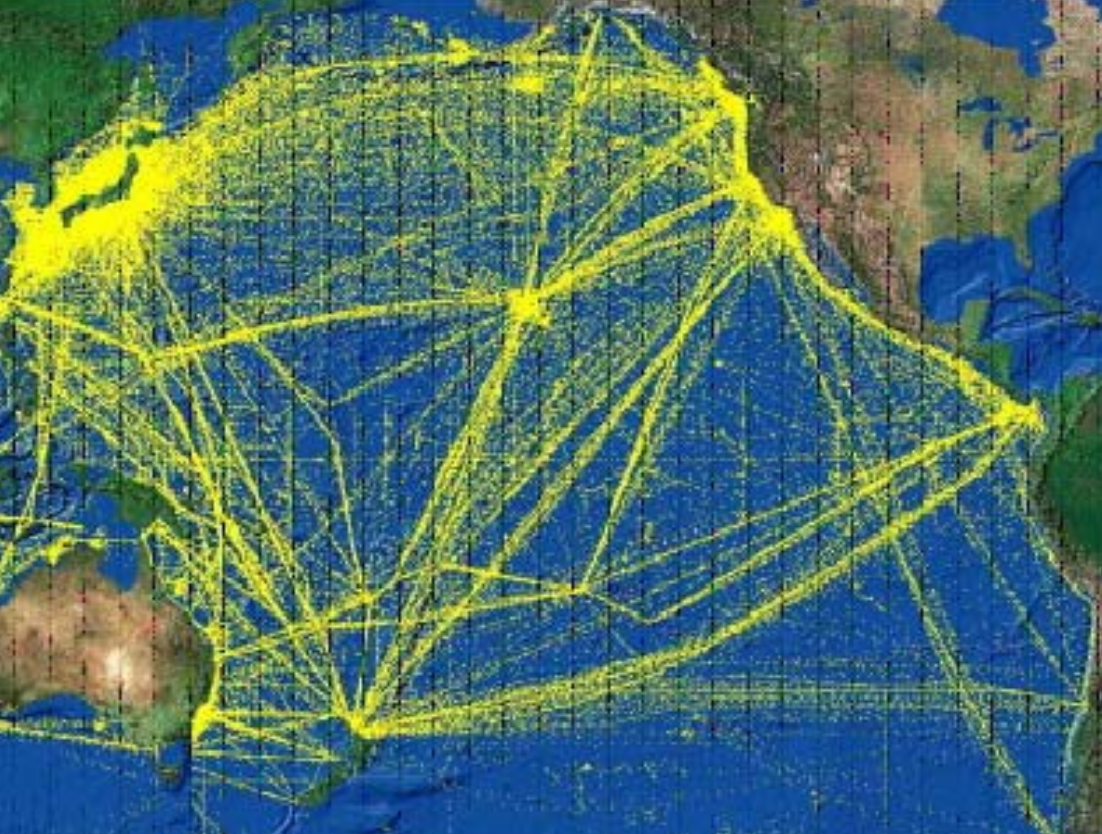
\includegraphics[width=0.5\textwidth]{pacific-traffic.png}
		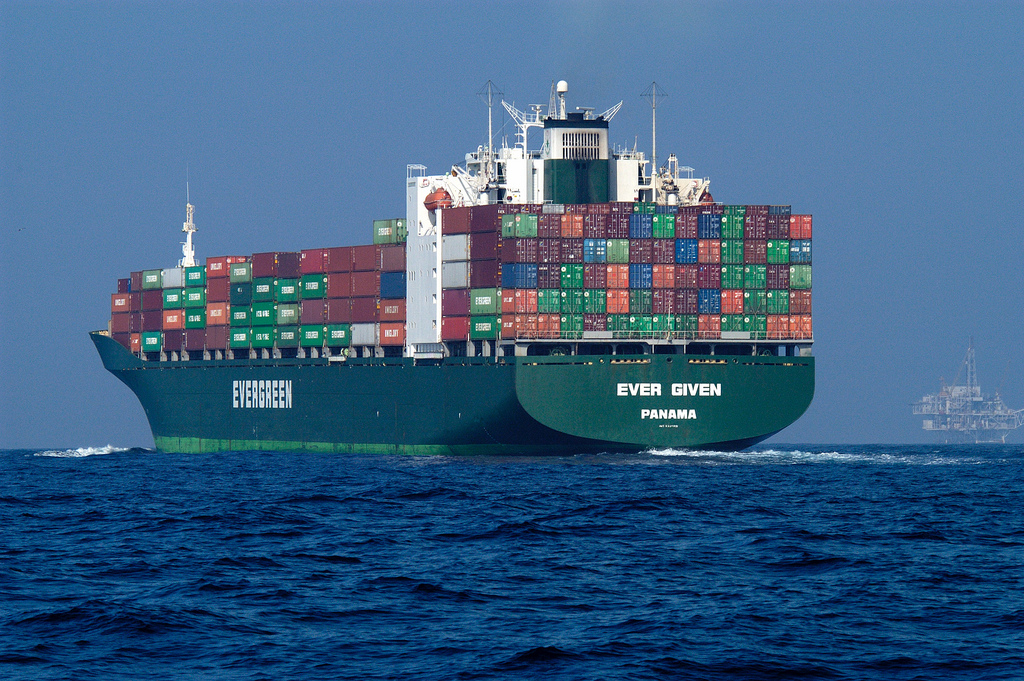
\includegraphics[width=0.5\textwidth]{container-ship.jpg}
		\caption{Rate of invasive species arrivals is correlated with \textbf{globalization} and \textbf{containerization}.}
	\end{figure}
\end{frame}

\begin{frame}{Kahalui Airport Pest Risk Assessment (KARA)}
	\begin{itemize}
		\item comprehensive inspection of all agricultural produces was performed on 130 days between September 2000 and July 2001
		\item specimens were identified to species
	\end{itemize}
	\begin{figure}
		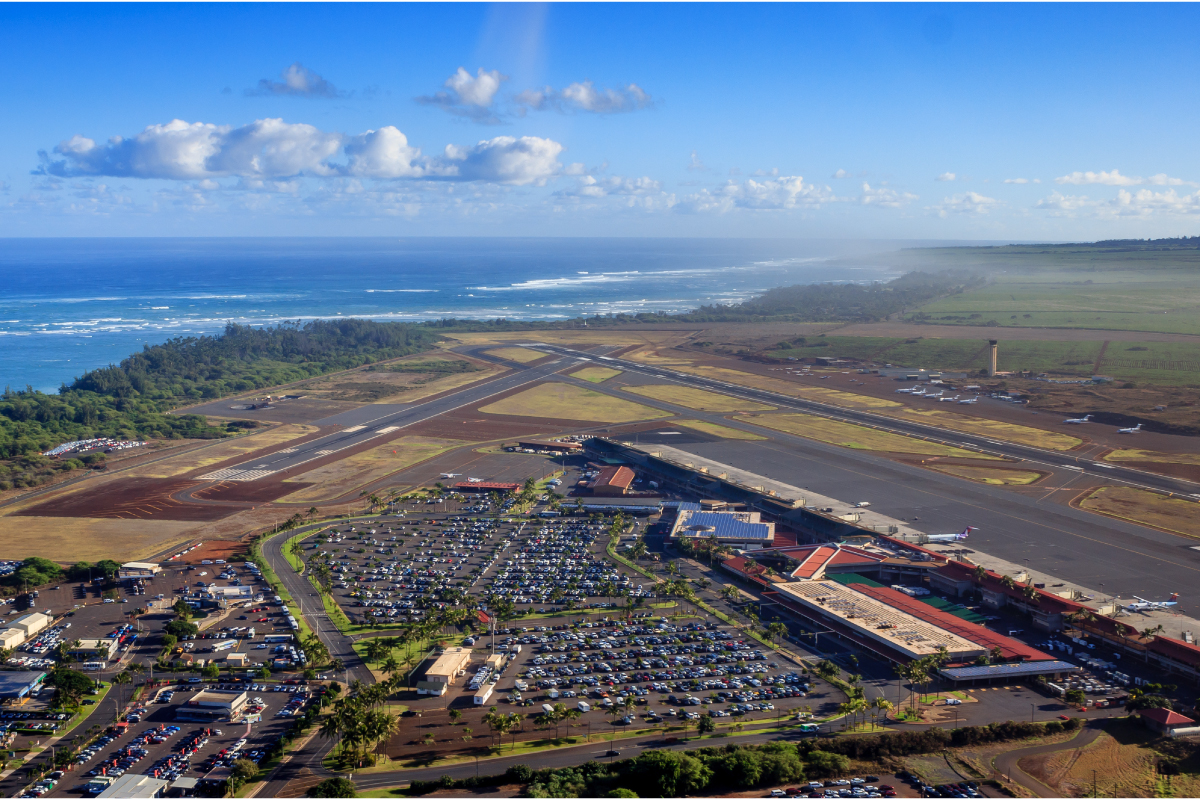
\includegraphics[height=0.35\textheight]{kahului-airport.jpg}
	\end{figure}
	\begin{itemize}
		\item 125 species of pest insects and 16 plant diseases not known to occur in Hawaii were intercepted at Kahului during the 130 days of KARA inspections
		\item \textbf{1 new invasive species arrived every day!}
	\end{itemize}
	\url{http://www.hawaiiag.org/PQ/KARA20Report20Final.pdf}
\end{frame}

\begin{frame}{Impact of invasive species on Guam}
	\begin{itemize}
		\item Almost all of Guam's pests are invasive species
		\item One third of the "100 World's Worst Invasive Species" list published by the IUCN Invasive Species Specialist Group  occur on Guam
	\end{itemize}
\end{frame}

\begin{frame}{Impediments to Dealing with Invasive Species on Guam}
	\begin{itemize}
		\item We suffer from the \textbf{Taxonomic Impediment}.
		\item Professional capacity is inadequate.
		\item Even when we manage to detect invasive species, our findings are rarely published in the scientific literature. 
		\item Arrivals of and impacts of invasive species impacts on small islands are grossly under-reported.
	\end{itemize}
\end{frame}

\begin{frame}{Major Biological Invasions on Guam}
	\begin{itemize}
		\item Brown treesnake (arrived around 1945)
			\begin{itemize}
			\item Killed most of Guam's birds and small mammals. Caused 7 bird extinctions.
			\end{itemize}
		\item Asian Cycad Scale (detected 2003)
			\begin{itemize}
				\item Threatens survival of Guam's endemic cycad, listed as the most numerous tree on Guam in the 2002 Forest Service survey.
			\end{itemize}
		\item Coconut Rhinoceros Beetle (detected 2007). 
			\begin{itemize}
			\item Threatens coconut palms, listed as the 2nd most numerous tree on Guam in the 2002 Forest Service survey.
			\end{itemize}
		\item Little Fire Ant (detected 2011)
			\begin{itemize}
		\item Threatens most animals remaining in Guam's forests.
			\end{itemize}
	\end{itemize}		
\end{frame}


\section{Brown treesnake}

\begin{frame}{Bird extinction by brown treesnake}
	\adjincludegraphics[height=0.85\textheight,center]{bts.jpg}
    \tiny{Courtesy of USGS}
\end{frame}

\begin{frame}{Forest Birds before BTS}
	\begin{figure}
		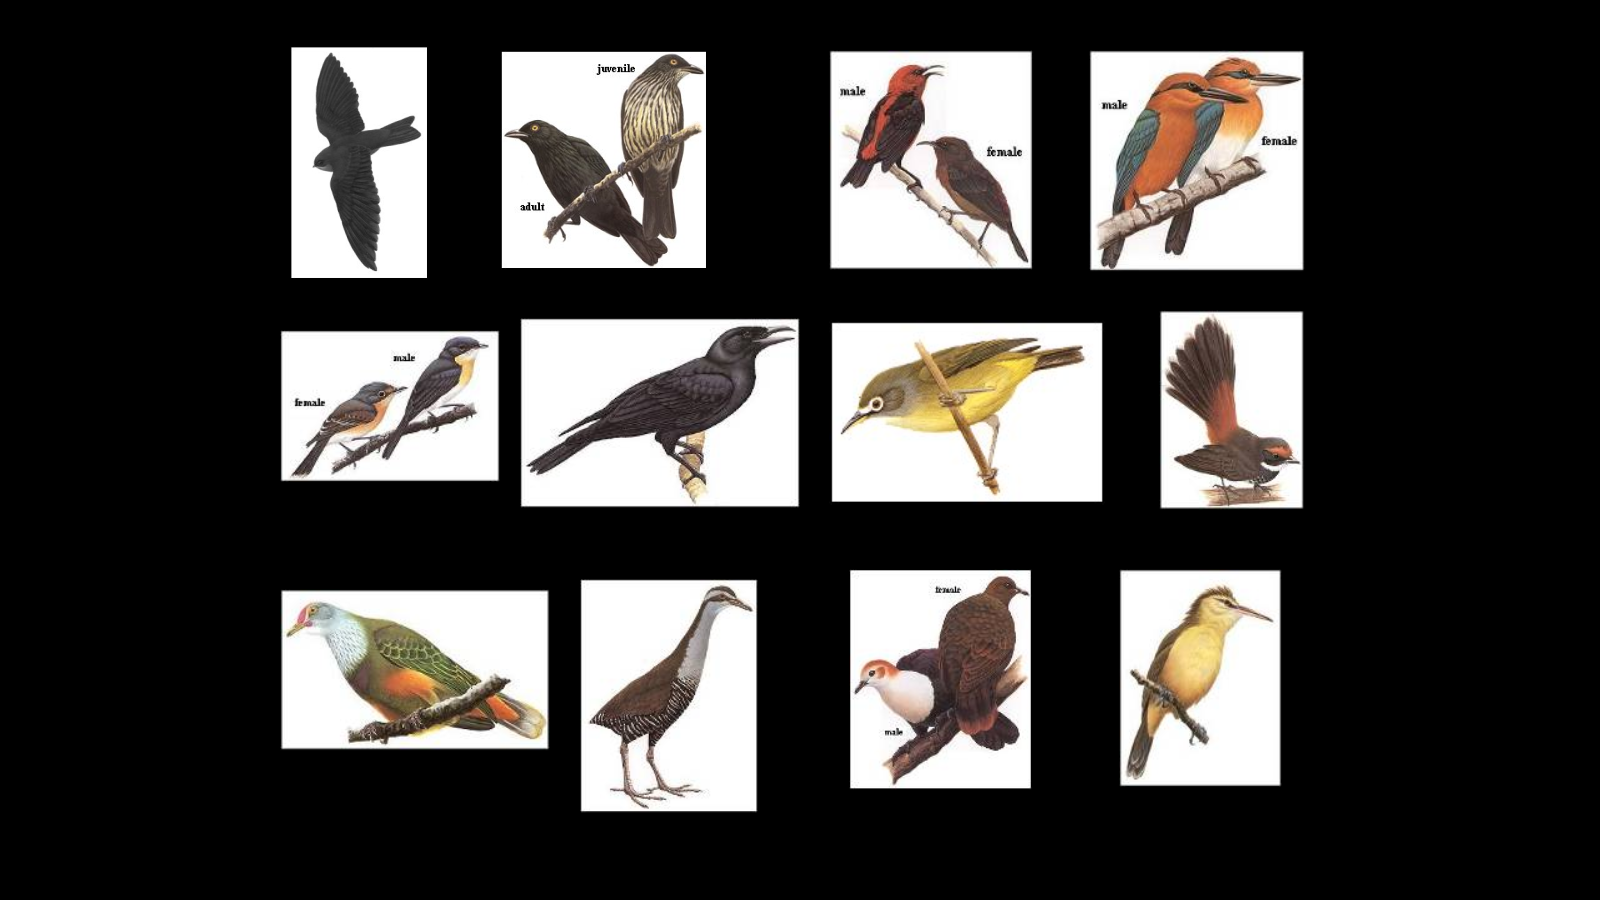
\includegraphics[height=0.8\textheight]{birds-before-bts.png}
	\end{figure}
\end{frame}

\begin{frame}{Forest Birds after BTS}
	\begin{figure}
		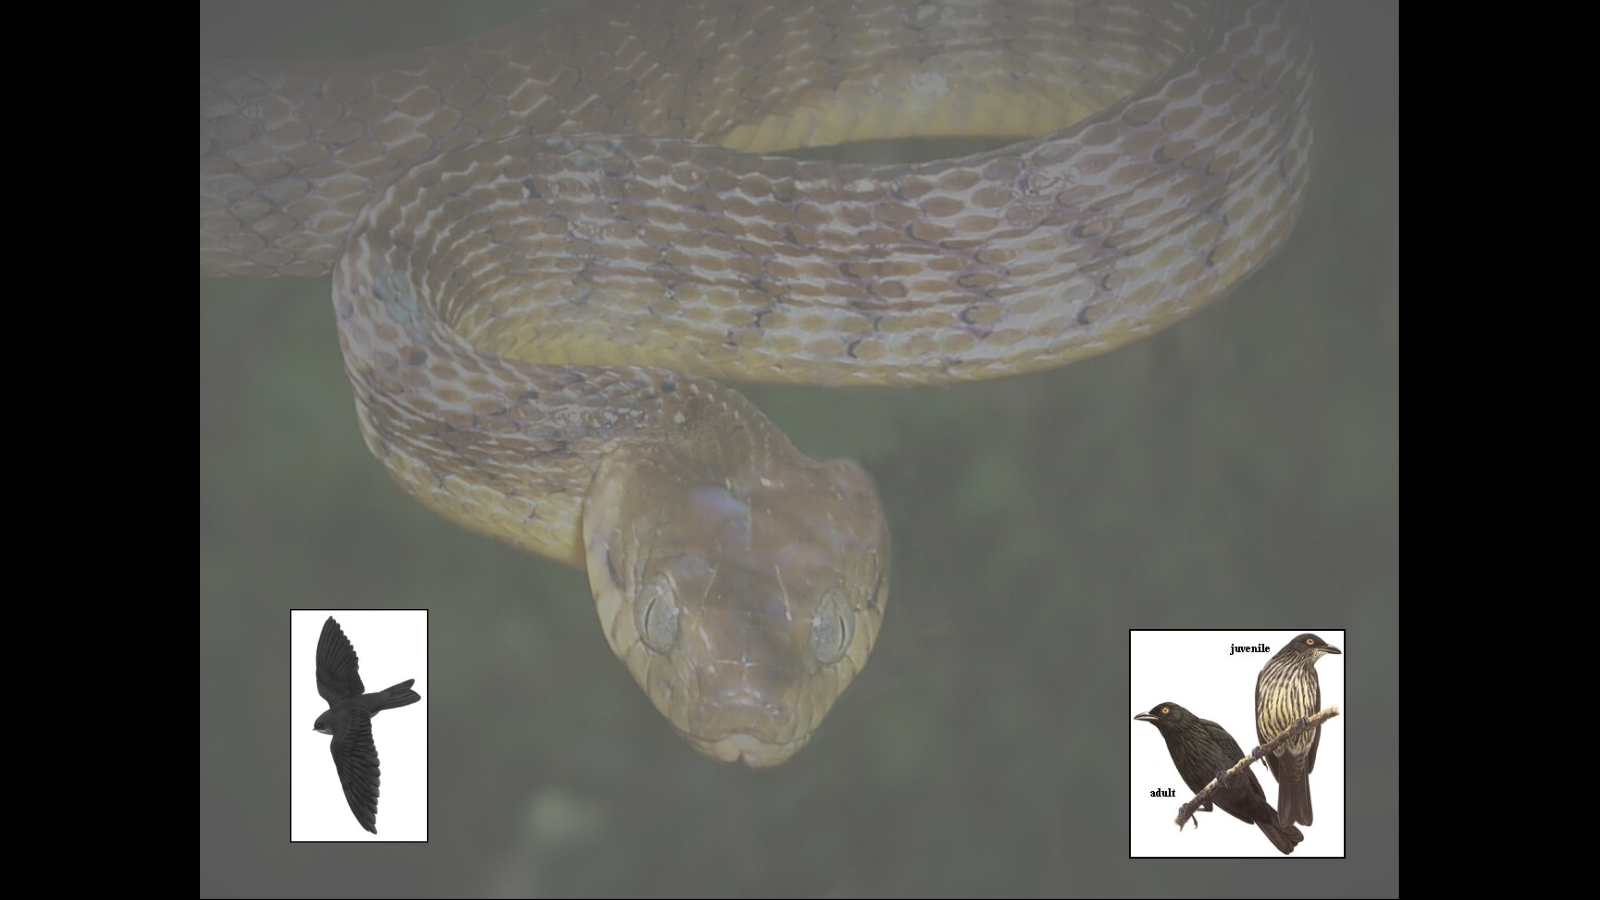
\includegraphics[height=0.8\textheight]{birds-after-bts.png}
	\end{figure}
\end{frame}

\begin{frame}{Loss of Ecosystem Services Provided by Birds}
	\begin{figure}
		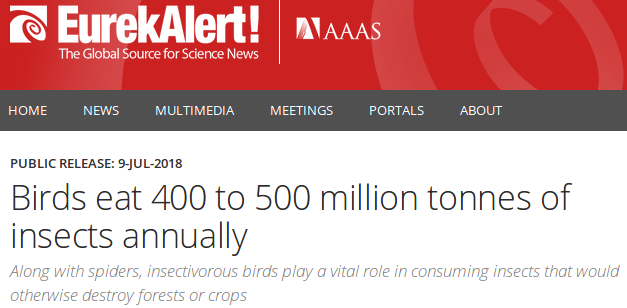
\includegraphics[height=0.5\textheight]{eureka-bird-loss.png}
	\end{figure}
"Birds are an endangered class of animals ... we must fear that the vital ecosystem services that birds provide - such as the suppression of insect pests - will be lost." says Nyffeler.
%\tiny{\url{https://link.springer.com/article/10.1007/s00114-018-1571-z#Sec10}}
\end{frame}

\begin{frame}{BTS - Current Status}
	\begin{itemize}
		\item Millions of dollars per year are spent on preventing BTS from leaving Guam.
		\item Some funds are being used for control methods development: snake-proof barriers and "pinkies on parachutes".
	\end{itemize}
\end{frame}

\section{Asian Cycad Scale}

\begin{frame}{07}
	\begin{figure}
		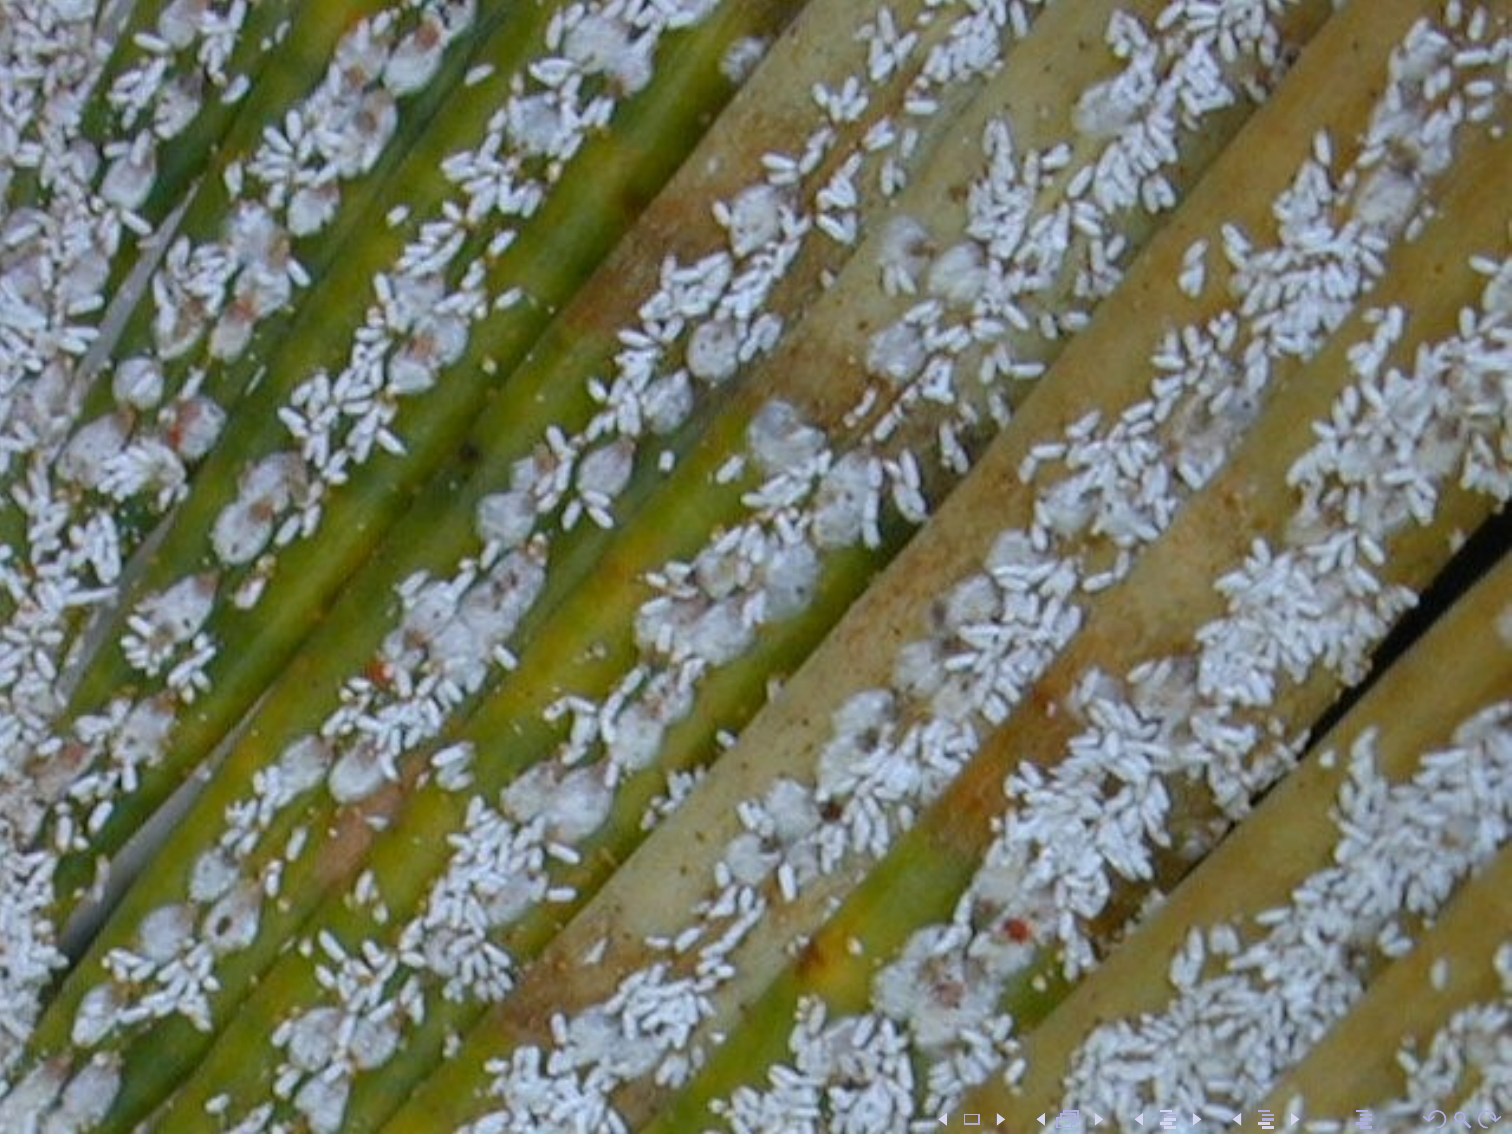
\includegraphics[height=0.7\textheight]{asian-cycad-scale/output-07.png}
		\caption{Asian cycad scale, \textit{Aulacaspis yasumatsui} (HEMIPTERA: DIASPIDIDAE)}
	\end{figure}
\end{frame}

\begin{frame}{Asian Cycad Scale - Origin and Pathway}
	\begin{itemize}
		\item Origin: Southeast Asia
		\item Florida
		\item Hawaii 1998
		\item Guam 2003
		\item Rota 2005?
		\item Palau 2005?
	\end{itemize}
\end{frame}

\begin{frame}{09}
\adjincludegraphics[width=\textwidth]{asian-cycad-scale/output-09.png}
\end{frame}

\begin{frame}{10}
\adjincludegraphics[width=\textwidth]{asian-cycad-scale/output-10.png}
\end{frame}

\begin{frame}{11}
\adjincludegraphics[width=\textwidth]{asian-cycad-scale/output-11.png}
\end{frame}

\begin{frame}{12}
\adjincludegraphics[width=\textwidth]{asian-cycad-scale/output-12.png}
\end{frame}

\begin{frame}{13}
\adjincludegraphics[width=\textwidth]{asian-cycad-scale/output-13.png}
\end{frame}

\begin{frame}{14}
\adjincludegraphics[width=\textwidth]{asian-cycad-scale/output-14.png}
\end{frame}

\begin{frame}{15}
\adjincludegraphics[width=\textwidth]{asian-cycad-scale/output-15.png}
\end{frame}

\begin{frame}{16}
\adjincludegraphics[width=\textwidth]{asian-cycad-scale/output-16.png}
\end{frame}

\begin{frame}{17}
\adjincludegraphics[width=\textwidth]{asian-cycad-scale/output-17.png}
\end{frame}

\begin{frame}{18}
\adjincludegraphics[width=\textwidth]{asian-cycad-scale/output-18.png}
\end{frame}

\begin{frame}{19}
\adjincludegraphics[width=\textwidth]{asian-cycad-scale/output-19.png}
\end{frame}

\begin{frame}{20}
\adjincludegraphics[width=\textwidth]{asian-cycad-scale/output-20.png}
\end{frame}

\begin{frame}{24}
\adjincludegraphics[width=\textwidth]{asian-cycad-scale/output-24.png}
\end{frame}

\begin{frame}{25}
\adjincludegraphics[width=\textwidth]{asian-cycad-scale/output-25.png}
\end{frame}

\begin{frame}{51}
\adjincludegraphics[width=\textwidth]{asian-cycad-scale/output-51.png}
\end{frame}

\begin{frame}{Massive mortality of \textit{Cycas micronesica} by invasive species}
	\note[item]{Invasive species have killed about 90\% of Guam's endemic \textit{C. micronesica} plants and the population is not recovering}
	\note[item]{\textit{C. micronesica} went from being the most numerous tree in Guam's forests in 2002 to being placed on the National Endangered Species list in 2016}
	\adjincludegraphics[height=0.9\textheight,center]{CAS.png}
\end{frame}

\begin{frame}{Asian Cycad Scale - Current Status on Guam}
	\begin{itemize}
		\item 90\% of Guam's endemic cycads have been killed by the scale and other invasive species
		\item Mature plants are protected by the biocontrol beetle, but no natural reproduction is occurring
		\item \textit{Cycas micronesica} placed on the US National Endangered Species List in 2015. (Was the most abundant tree on Guam in 2002.)
	\end{itemize}
\end{frame}

\section{Coconut Rhinoceros Beetle}

\begin{frame}{Coconut rhincoceros beetle}
\adjincludegraphics[width=\textwidth]{crb-climate-change-connection/outputname-02.png}
\end{frame}

\begin{frame}{Geographic Distribution of Coconut Rhinoceros Beetle}
\adjincludegraphics[width=\textwidth]{crb_map.png} \\
\url{http://aubreymoore.github.io/crbdist/mymap.html}.
\end{frame}

\begin{frame}{Coconut Rhinoceros Beetle Life Cycle}
	\adjincludegraphics[height=0.9\textheight,center]{crb_life_cycle2_cropped.png}
\end{frame}

\begin{frame}{Coconut rhincoceros beetle}
\adjincludegraphics[width=\textwidth]{crb-climate-change-connection/outputname-08.png}
\end{frame}

\begin{frame}{Coconut rhincoceros beetle}
\adjincludegraphics[width=\textwidth]{crb-climate-change-connection/outputname-04.png}
\end{frame}

\begin{frame}{Coconut rhincoceros beetle}
\adjincludegraphics[width=\textwidth]{crb-climate-change-connection/outputname-05.png}
\end{frame}

\begin{frame}{Coconut rhincoceros beetle}
\adjincludegraphics[width=\textwidth]{crb-climate-change-connection/outputname-09.png}
\end{frame}

\begin{frame}{Coconut rhincoceros beetle}
\adjincludegraphics[width=\textwidth]{crb-climate-change-connection/outputname-10.png}
\end{frame}

\begin{frame}{Coconut Rhinoceros Beetle - Current Status on Guam}
	\begin{itemize}
		\item Mature coconuts and other palms are rapidly being killed by an uncontrolled outbreak of CRB-G which was triggered by Typhoon Dolpine in 2016
		\item Damage estimates are not available. History from Palau suggests that we will loose 50\% or more of our palms if the outbreak is not contoled.
		\item A search for an effective biological control agent, most likely a new isolate of Oryctes nudivirus is under way.
		\item If current outbreaks of CRB-G cannot be controled, CRB-G will spread to other islands and possibly the Americas.
	\end{itemize}
\end{frame}

\begin{frame}{LFA - Prognosis for Guam}
	\begin{itemize}
		\item A search for an effective biological control agent, most likely a new isolate of \textit{Oryctes rhinoceros} nudivirus is under way.
	\end{itemize}
\end{frame}

\begin{frame}{Coconut rhincoceros beetle}
\adjincludegraphics[width=\textwidth]{crb-climate-change-connection/outputname-14.png}
\end{frame}

\begin{frame}{Coconut rhincoceros beetle}
\adjincludegraphics[width=\textwidth]{crb-climate-change-connection/outputname-13.png}
\end{frame}

\begin{frame}{Coconut rhincoceros beetle}
\adjincludegraphics[width=\textwidth]{crb-climate-change-connection/outputname-15.png}
\end{frame}

\section{Little Fire Ant}

\begin{frame}{LFA - Biology}
	\begin{figure}
	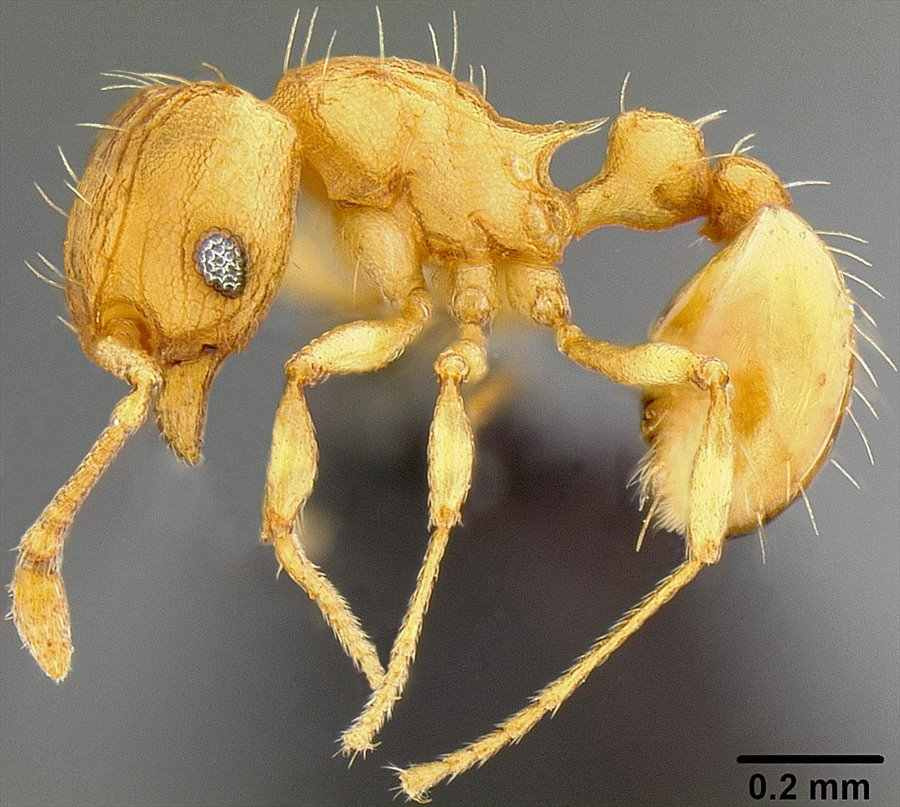
\includegraphics[height=0.6\textheight]{lfa.jpg}
	\caption{Little fire ant, \textit{Wasmannia auropunctata} (HYMENOPTERA: FORMICIDAE)}
	\end{figure}
	\begin{itemize}
		\item Forms supercolonies with multiple queens
		\item Nests in trees and on ground
	\end{itemize}
\end{frame}

\begin{frame}{LFA - Biology}
\begin{figure}
	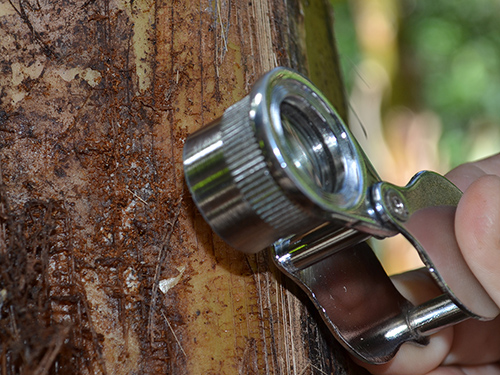
\includegraphics[width=0.5\textwidth]{lfa2small.jpg}
	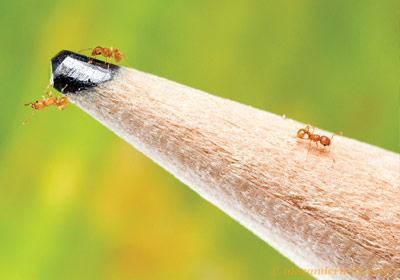
\includegraphics[width=0.5\textwidth]{lfa-pencil.jpg}
	\caption{Little fire ants are little :)}
\end{figure}
\end{frame}

\begin{frame}{LFA - Biology}
\begin{figure}
	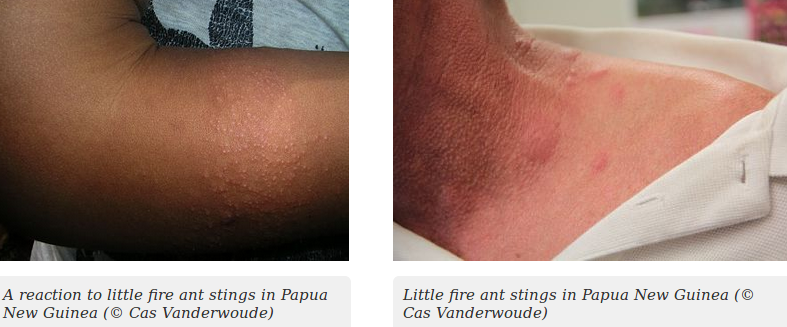
\includegraphics[width=\textwidth]{lfa-stings.png}
\end{figure}
\end{frame}

\begin{frame}{LFA - Biology}
\begin{figure}
	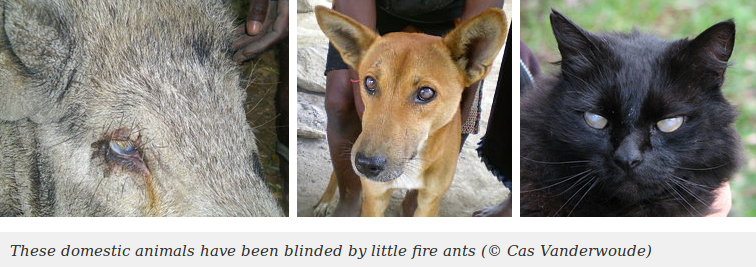
\includegraphics[width=\textwidth]{lfa-eyes.png}
\end{figure}
\end{frame}

\begin{frame}{LFA - Biology}
\begin{figure}
	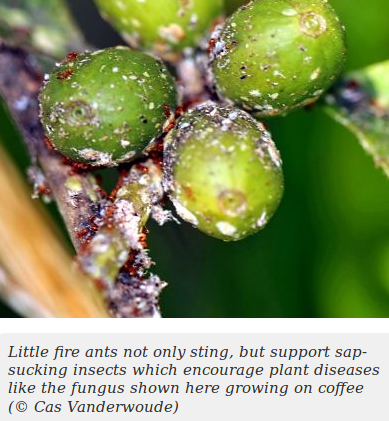
\includegraphics[height=0.85\textheight]{lfa-hemiptera.png}
\end{figure}
\end{frame}

\begin{frame}{Little Fire Ant - Origin and Pathway}
	\begin{itemize}
		\item Origin: South America
		\item Florida 1920s
		\item Hawaii 1999
		\item Guam 2011
		\item Yap 2017
	\end{itemize}
\end{frame}

\begin{frame}{LFA - Detection on Guam}
	\begin{figure}	
		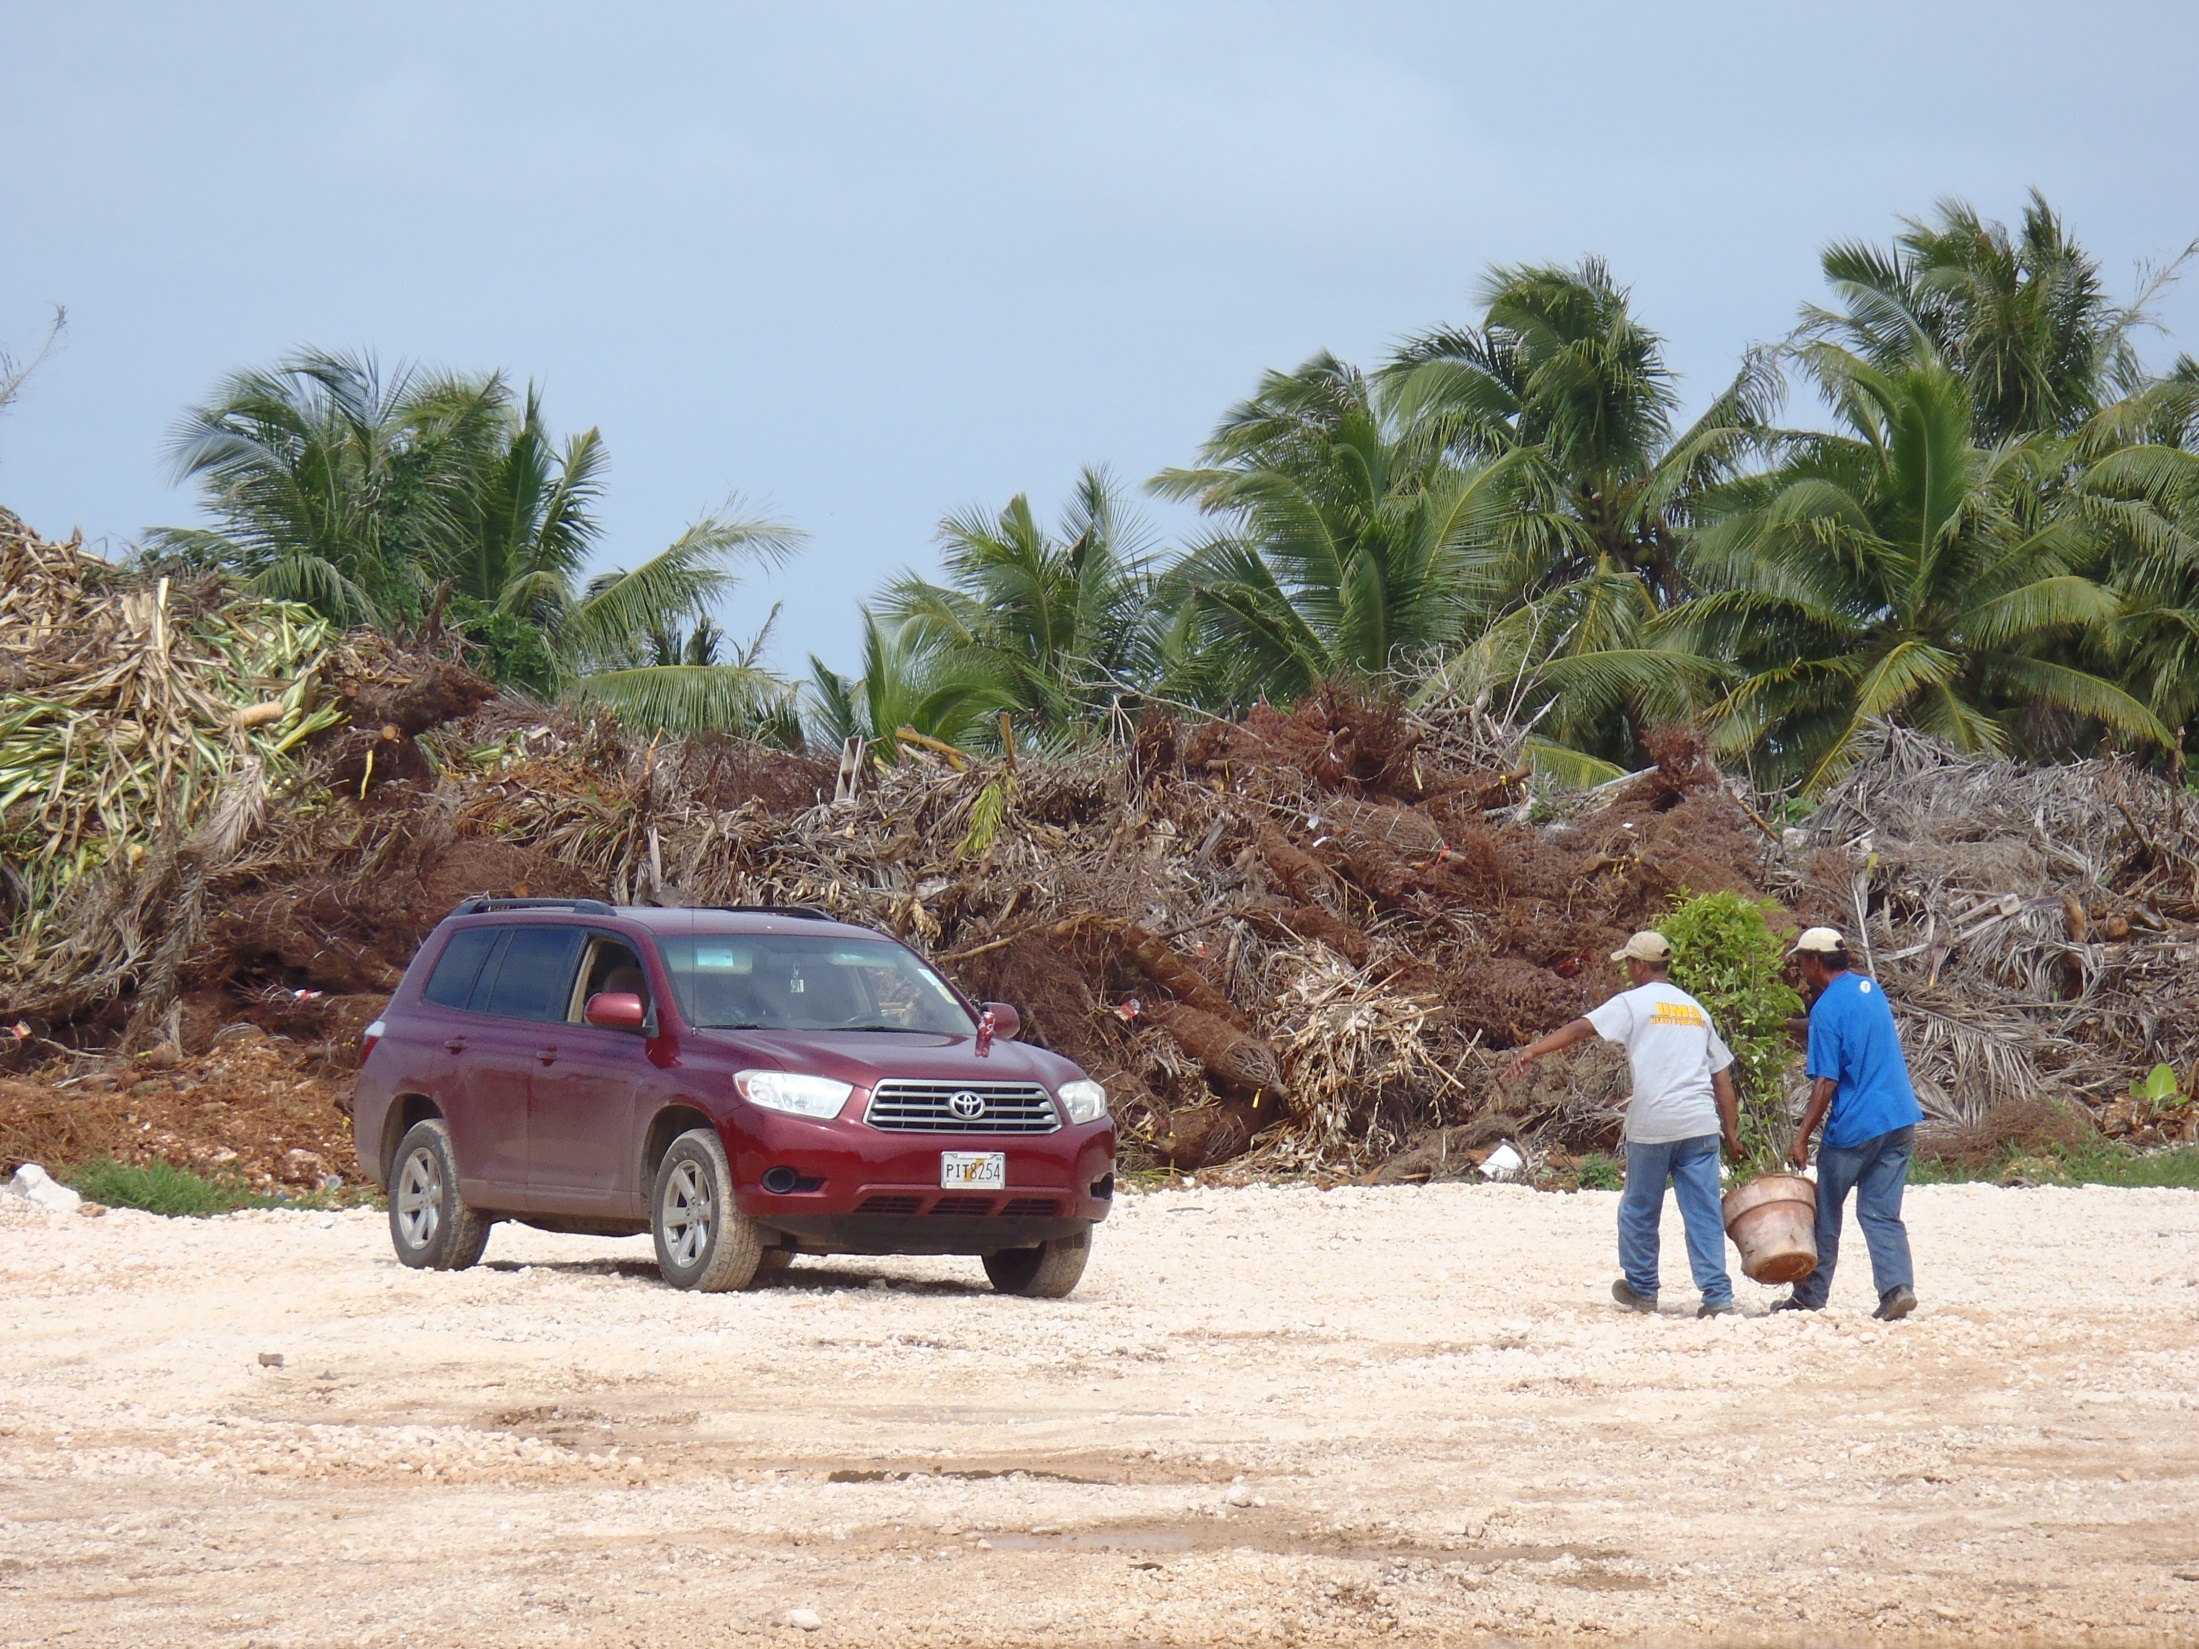
\includegraphics[height=.75\textheight]{lfa-dump.png}
		\caption{LFA discovered by CRB crew at Primo Greenwaste Dump Site in Yigo in 2011.}
	\end{figure}
\end{frame}

\begin{frame}{LFA - Current Status on Guam}
	\begin{itemize}
		\item Eradication from Guam is not feasable
		\item LFA occurs at 20+ dispersed sites on Guam and continues to spread
		\item Effective ant baits and application methods are available for local control programs
	\end{itemize}
\end{frame}

\begin{frame}{LFA - Prognosis for Guam}
	\begin{itemize}
		\item There are no known biocontrol agents for island-wide control of LFA
		\item Will impact quality of life for humans and pets
		\item Possible impacts on tourism
		\item Impacts on natural ecosystems are unpredicable
	\end{itemize}
\end{frame}


\begin{frame}{}
\adjincludegraphics[width=\textwidth]{asian-cycad-scale/output-53.png}
\end{frame}

\end{document}
